%%%%%%%%%%%%%%%%%%%%%%%%%%%%%%%%%%%%%%%%%%%%%%%%%%%%%%%%%%%%%%%%%%%%%%%%%%%%
% AGUJournalTemplate.tex: this template file is for articles formatted with LaTeX
%
% This file includes commands and instructions
% given in the order necessary to produce a final output that will
% satisfy AGU requirements, including customized APA reference formatting.
%https://www.overleaf.com/project/5f1175280f47d00001f0b4dd
% You may copy this file and give it your
% article name, and enter your text.
%
%
% Step 1: Set the \documentclass
%
%

%% To submit your paper:
\documentclass[draft]{agujournal2019}
\usepackage{url} %this package should fix any errors with URLs in refs.
\usepackage{lineno}
\usepackage[ignoremode,finalnew]{trackchanges} %for better track changes. finalnew option will compile document with changes incorporated.
\usepackage{soul}
\linenumbers
\newcommand{\cledit}[1]{{\textcolor{violet}{#1}}} 
\usepackage{setspace}
%\doublespacing
\newcommand{\pkedit}[1]{{\textcolor{blue}{#1}}} 


%%%%%%%
% As of 2018 we recommend use of the TrackChanges package to mark revisions.
% The trackchanges package adds five new LaTeX commands:
%
%  \note[editor]{The note}
%  \annote[editor]{Text to annotate}{The note}
%  \add[editor]{Text to add}
%  \remove[editor]{Text to remove}
%  \change[editor]{Text to remove}{Text to add}
%
% complete documentation is here: http://trackchanges.sourceforge.net/

\addeditor{eds}
\tcignore{\cite}{1}{0}
\tcignore{\citeA}{1}{0}

%%%%%%%

\draftfalse

%% Enter journal name below.
%% Choose from this list of Journals:
%
% JGR: Atmospheres
% JGR: Biogeosciences
% JGR: Earth Surface
% JGR: Oceans
% JGR: Planets
% JGR: Solid Earth
% JGR: Space Physics
% Global Biogeochemical Cycles
% Geophysical Research Letters
% Paleoceanography and Paleoclimatology
% Radio Science
% Reviews of Geophysics
% Tectonics
% Space Weather
% Water Resources Research
% Geochemistry, Geophysics, Geosystems
% Journal of Advances in Modeling Earth Systems (JAMES)
% Earth's Future
% Earth and Space Science
% Geohealth
%
% ie, \journalname{Water Resources Research}

\journalname{Geophysical Research Letters}


\begin{document}

%% ------------------------------------------------------------------------ %%
%  Title
%
% (A title should be specific, informative, and brief. Use
% abbreviations only if they are defined in the abstract. Titles that
% start with general keywords then specific terms are optimized in
% searches)
%
%% ------------------------------------------------------------------------ %%

% Example: \title{This is a test title}

\title{Limited influence of localized tropical sea-surface temperatures on moisture transport into the Arctic}



%% ------------------------------------------------------------------------ %%
%
%  AUTHORS AND AFFILIATIONS
%
%% ------------------------------------------------------------------------ %%

% Authors are individuals who have significantly contributed to the
% research and preparation of the article. Group authors are allowed, if
% each author in the group is separately identified in an appendix.)

% List authors by first name or initial followed by last name and
% separated by commas. Use \affil{} to number affiliations, and
% \thanks{} for author notes.
% Additional author notes should be indicated with \thanks{} (for
% example, for current addresses).

% Example: \authors{A. B. Author\affil{1}\thanks{Current address, Antartica}, B. C. Author\affil{2,3}, and D. E.
% Author\affil{3,4}\thanks{Also funded by Monsanto.}}

\authors{Etienne Dunn-Sigouin\affil{1}, Camille Li\affil{1}, Paul J. Kushner\affil{2}}


% \affiliation{1}{First Affiliation}
% \affiliation{2}{Second Affiliation}
% \affiliation{3}{Third Affiliation}
% \affiliation{4}{Fourth Affiliation}

\affiliation{1}{Geophysical Institute, University of Bergen and Bjerknes Centre for Climate Research, Bergen, Norway}
\affiliation{2}{Department of Physics, University of Toronto, Toronto, Ontario, Canada}
%(repeat as many times as is necessary)

%% Corresponding Author:
% Corresponding author mailing address and e-mail address:

% (include name and email addresses of the corresponding author.  More
% than one corresponding author is allowed in this LaTeX file and for
% publication; but only one corresponding author is allowed in our
% editorial system.)

% Example: \correspondingauthor{First and Last Name}{email@address.edu}

\correspondingauthor{Etienne Dunn-Sigouin}{edu061@uib.no}

%% Keypoints, final entry on title page.

%  List up to three key points (at least one is required)
%  Key Points summarize the main points and conclusions of the article
%  Each must be 140 characters or fewer with no special characters or punctuation and must be complete sentences

% Example:
% \begin{keypoints}
% \item	List up to three key points (at least one is required)
% \item	Key Points summarize the main points and conclusions of the article
% \item	Each must be 140 characters or fewer with no special characters or punctuation and must be complete sentences
% \end{keypoints}

\begin{keypoints}

\item  Arctic moisture transport is dominated by transient planetary waves in aquaplanet model driven by zonally uniform boundary conditions

\item Tropical sea-surface temperature anomalies affect Arctic moisture transport mostly via changes in water vapor 

\item Localized tropical perturbations alter Arctic moisture transport more than uniform perturbations for cooling but not warming


\end{keypoints}

%% ------------------------------------------------------------------------ %%
%
%  ABSTRACT and PLAIN LANGUAGE SUMMARY
%
% A good Abstract will begin with a short description of the problem
% being addressed, briefly describe the new data or analyses, then
% briefly states the main conclusion(s) and how they are supported and
% uncertainties.

% The Plain Language Summary should be written for a broad audience,
% including journalists and the science-interested public, that will not have 
% a background in your field.
%
% A Plain Language Summary is required in GRL, JGR: Planets, JGR: Biogeosciences,
% JGR: Oceans, G-Cubed, Reviews of Geophysics, and JAMES.
% see http://sharingscience.agu.org/creating-plain-language-summary/)
%
%% ------------------------------------------------------------------------ %%

%% \begin{abstract} starts the second page


\begin{abstract}



Arctic moisture transport is dominated by planetary-scale waves in reanalysis \remove[eds]{data}. Planetary waves are influenced by localized Sea-Surface Temperature (SST) features such as the tropical warm pool. Here, \change[eds]{a simplified}{an} aquaplanet model is used to clarify the link between tropical SST anomalies and \remove[eds]{zonally integrated} Arctic moisture transport. In a zonally uniform \remove{model} setup with no climatological east-west gradients, Arctic moisture transport is dominated by transient planetary waves, as in reanalysis. Warming tropical SSTs \add[eds]{by heating the ocean} strengthens Arctic moisture transport, mediated mostly by changes in water vapor rather than eddies. This strengthening occurs \remove[eds]{regardless of} whether the tropical warming is zonally uniform or localized. Cooling tropical SSTs weakens Arctic moisture transport; however, unlike warming, the pattern matters, with localized cooling producing stronger transport changes owing to non-linear feedbacks in the surface energy budget. Thus, \add[eds]{the simulations show that} localized tropical SST anomalies \remove[eds]{can} influence Arctic moisture transport differently than uniform anomalies, but only in cooling scenarios.



\end{abstract}


\section*{Plain Language Summary} 

Northward transport of water vapor strongly influences Arctic climate. Most of the transport is accomplished by atmospheric waves with large east-west scale extending around the earth. These waves can be generated by warm ocean waters in the western tropical Pacific. Here, a simplified climate model with an ocean covered surface is used to clarify the processes linking the tropical ocean and Arctic moisture transport. Arctic transport in the model is accomplished by waves that are similar to observations, suggesting it is a useful tool. Warming the tropical ocean strengthens Arctic transport similarly whether the warming pattern is concentrated in a specific location or spread out equally at all longitudes. The strengthening results mostly from an increase in water vapor arising from an increase in the holding capacity of the atmosphere at warmer temperatures. Cooling the tropical ocean weakens Arctic transport but, unlike warming, cooling concentrated in a specific location weakens the transport more than if it is spread out equally at all longitudes. The different responses arise because ocean temperatures adjust differently to warming versus cooling.  Thus, localized cooling of tropical ocean temperatures appears to be a special case in terms of its influence on moisture transport into the Arctic.

%% ------------------------------------------------------------------------ %%
%
%  TEXT
%
%% ------------------------------------------------------------------------ %%

%%% Suggested section heads:
% \section{Introduction}
%
% The main text should start with an introduction. Except for short
% manuscripts (such as comments and replies), the text should be divided
% into sections, each with its own heading.

% Headings should be sentence fragments and do not begin with a
% lowercase letter or number. Examples of good headings are:

% \section{Materials and Methods}
% Here is text on Materials and Methods.
%
% \subsection{A descriptive heading about methods}
% More about Methods.
%
% \section{Data} (Or section title might be a descriptive heading about data)
%
% \section{Results} (Or section title might be a descriptive heading about the
% results)
%
% \section{Conclusions}


\section{Introduction}

Poleward atmospheric moisture transport exerts a strong influence on Arctic climate, causing surface warming, sea-ice melt and ocean freshening \cite{Doyle2011, Kapsch2013, Park2015, SerrezeBarry2014, Vihma2016, WoodsCaballero2016, Johansson2017, Liu2018}.  This moisture transport is accomplished by atmospheric waves, of which the planetary-scale waves are critical for Arctic surface impacts \cite{BaggettLee2015, GraversenBurtu2016, Heiskanen2020, Lee2019, PapritzDunnSigouin2020}. Planetary wave trains are strongly affected by localized sea-surface temperature (SST) features such as the tropical warm pool, with signals reaching well into the midlatitudes \cite{HorelWallace1981, PalmerMansfield1984, Ding2014}. However, how the zonal (east-west) structure of SST anomalies influences Arctic moisture transport remains unclear.

Localized warming of tropical SSTs could enhance Arctic moisture transport by exciting planetary waves. For example, anomalously warm SSTs in the western Pacific warm pool trigger atmospheric convection, resulting in localized diabatic heating and divergent flow aloft, which in turn generates poleward propagating planetary waves \cite{HoskinsKaroly1981, SardeshmukhHoskins1988, Branstator2014}. Planetary waves of this kind are quasi-stationary and have been suggested to transport moisture into the Arctic either directly or indirectly by interacting with transient eddies \cite{Lee2014, Yoo2012a, BaggettLee2015, Baggett2016, Goss2016, Baggett2017, Lee2019, ParkLee2019}. Indeed, sub-seasonal to decadal variability in warm pool convection has been linked to corresponding variability in Arctic moisture transport and surface temperature in observations \cite{Lee2011a, Lee2012, Yoo2011, Gong2017}.


Warming tropical SSTs could also drive Arctic moisture transport via processes that rely on changes in the zonal-mean state rather than in quasi-stationary planetary waves. For example, localized SST anomalies in the western Pacific produce a zonally uniform atmospheric temperature change in the tropics \cite{YulaevaWallace1994,Sobel2001} that can modify transient eddies and their associated energy transport in the extratropics \cite{Robinson2002, Seager2003, LheureuxThompson2006}. Tropical atmospheric temperatures are also tightly coupled to water vapor \cite{WentzSchabel2000, Trenberth2005}, so changes in Arctic moisture transport might be expected to scale with the Clausius-Clapeyron relationship, in a manner similar to other aspects of the climate system under global warming \cite{HeldSoden2006, LorenzDeWeaver2007, Seager2010}. 


In addition to how moisture transport changes driven by tropical SST anomalies are communicated to the Arctic, we must also consider that the effects of cooling (e.g., La Ni\~na) may differ from those of warming (e.g., El Ni\~no). For example, cooling produces a larger SST change per unit energy perturbation because, unlike heating, the resulting energy imbalance is not efficiently offset by evaporation \cite{Shin2017}. Cooling also induces changes in surface cloud radiative forcing that amplify the cooling \cite{Shaw2015}. Thus, cooling could more efficiently perturb tropical SSTs than warming, leading to a more pronounced change in the zonal-mean state and a greater change in Arctic moisture transport. Moreover, tropical convection depends \change[eds]{non-linearly}{sensitively} on the absolute value of SST, so equal but opposite SST anomalies could excite different quasi-stationary planetary waves \cite{Hoerling1997} that result in different Arctic moisture transport.



To elucidate how tropical SSTs affect moisture transport into the Arctic, and which structural features of SST anomaly patterns are most important, we carry out a series of perturbation experiments using a slab-ocean aquaplanet model. The model allows us to clarify the processes governing observed zonally integrated Arctic moisture transport (section 3.1), as well as the role of localized tropical SST anomalies induced by warming or cooling in driving changes in moisture transport (Section 3.2). This, to our knowledge, provides a novel testbed for isolating the role of tropical SSTs on Arctic moisture transport mediated by planetary waves. The results suggest that an ongoing focus on transient, high-latitude, planetary waves is warranted, and show a concrete but limited influence of localized SST anomalies on zonally integrated Arctic moisture transport arising from tropical cooling (Section 4).




\section{Model, experiments and diagnostics}

The National Center for Atmospheric Research Community Atmospheric Model version 5 \cite<NCAR CAM5,>{Neale2010} is used. The atmosphere has a horizontal resolution of 1$^{\circ}$ latitude by 1.25$^{\circ}$ longitude, has 30 vertical hybrid-sigma levels and is coupled to a slab ocean. The control simulation is forced with zonally uniform boundary conditions following the Tropical Rain belts with an Annual Cycle and continent Model Intercomparison Project protocol \cite<TRACMIP,>{Voigt2016}. Specifically, the model is forced with present-day seasonal and diurnal cycles of insolation and concentrations of greenhouse gases, the slab ocean depth is set to 30 m, sea ice is turned off (SSTs can drop below freezing), zonal-mean ozone is prescribed following \citeA{BlackburnHoskins2013}\cledit{,} and a time-independent ocean heat flux convergence (termed the ``Q-flux") is prescribed to approximate the observed climatological zonal-mean \cite<equation 3 and Table 2 in>{Voigt2016}. The control simulation is spun up for 10 years and the next 40 years are used for analysis. The control and other simulations are compared to ERA-Interim data from 1979-2017 \cite{Dee2011}.


We investigate the impact of tropical SSTs on moisture transport into the Arctic by imposing time-independent Q-flux perturbations in the tropics, which generate diabatic heating anomalies and extratropical circulation responses. Experiment L+ imposes a localized Q-flux perturbation centred on the equator with a spatial scale of approximately 90$^\circ$ longitude and 30$^\circ$ latitude (Fig. 1a). The exact pattern is taken from equation 5 in \citeA{NealeHoskins2000}:



$$
Q( \lambda, \phi)= \left\{ \begin{array}{rl}
\chi \cos^{2} \big( \frac{\pi}{2} \big[ \frac{\lambda}{\lambda_{d}} \big] \big) \cos^{2} \big( \frac{\pi}{2} \big[ \frac{\phi}{\phi_{d}} \big] \big) &\mbox{: $-\lambda_{d} < \lambda < \lambda_{d} $, $-\phi_{d} < \phi < \phi_{d} $ }  \\
 0 &\mbox{: otherwise} 
        \end{array} \right.
 $$
 

\noindent
where $\lambda$ denotes longitude, $\phi$ denotes latitude, and the spatial extent of the perturbation is set by $\lambda_{d} = \pi / 2$ and $\phi_{d} = \pi /6$. The magnitude $\chi = 150$ Wm$^{-2}$ is chosen to resemble the annual-mean east-west difference in ocean heat flux convergence across the equatorial Pacific in reanalysis. We have confirmed that the results are similar for different choices of the spatial scale $\lambda_{d}$ and that the resulting Arctic stationary waves have comparable amplitude to reanalysis (Fig. S1 and S2). Experiment U+ imposes a zonally uniform Q-flux perturbation with the same total heat input as in experiment L+, but distributed equally over all longitudes (Fig. 1c). Thus, experiments U+ and L+ input identical amounts of globally integrated energy into the slab ocean. Additional experiments are performed where the sign of the Q-flux perturbation is reversed (L-, U-), the magnitude is doubled (2L+, 2U+), and a zonal wavenumber $k=1$ pattern with amplitude 75 Wm$^{-2}$ is imposed \cite<L$_{k1}$, equation 6 in >{NealeHoskins2000}. The last experiment inputs zero globally integrated energy into the slab ocean. The experiments are branched from the last day of the control simulation, spun up for 10 years and the next 40 years are used for analysis. 



Figure \ref{f1} shows annual-mean SST anomalies relative to the control simulation (shading) resulting from the Q-flux perturbations (purple contours). The SST warming (cooling) generally follows the pattern of heat input (output) by the Q-flux forcing. However, localized heat removal (Fig. \ref{f1}b) produces stronger SST anomalies than localized heat input (Fig. \ref{f1}a), and dominates the response when both forcings are present (Fig. \ref{f1}f). This asymmetry arises due to non-linear feedbacks in the surface energy budget \cite{Shaw2015, Shin2017} and becomes apparent when the Q-flux perturbations are larger (compare Fig. \ref{f1}a,b and c,d). This asymmetry will be useful for understanding the Arctic moisture transport responses discussed later. The tropical SST responses are communicated to the tropical atmosphere via changes in convection, reflected in changes in vertically integrated diabatic heating (Fig. S3). This, in turn, results in the generation or attenuation of quasi-stationary planetary waves \cite{SardeshmukhHoskins1988} \remove[eds]{which depends sensitively on the absolute value of tropical SST \cite{Hoerling1997}. We note, however, that these experiments do not include climatological zonal asymmetries from the presence of land and orography, which could modify the poleward propagation of planetary waves and attendant Arctic moisture transport \cite{Simmons1983, TingSardeshmuhk1993, Goss2016}. Our results should be interpreted with this caveat in mind.}



\add[eds]{These experiments do not include climatological zonal asymmetries from the presence of land and orography and so the resulting changes in Arctic planetary waves and moisture transport should be interpreted with certain caveats in mind. For example, zonal asymmetries can modify the extratropical waveguide and poleward propagation of planetary waves} \cite{Simmons1983, TingSardeshmuhk1993}. \add[eds]{Moreover, a given SST anomaly can generate different planetary waves depending on its location relative to a zonally varying background state. This is because the planetary wave source depends on tropical convection, which is sensitive to the absolute value of SST} \cite{Hoerling1997} \add[eds]{and the location of this convection relative to the climatological waveguide} \cite{Branstator2014}. \add[eds]{Nevertheless, these experiments represent a first step in understanding the link between tropical SST anomalies and Arctic moisture transport.}




We diagnose daily vertically and zonally integrated eddy moisture transport as a function of zonal wavenumber following \citeA{GraversenBurtu2016}: 

$$
\langle [v^{*}q^{*}] \rangle  =  \sum_{k}  \int_{0}^{2\pi} \int_{0}^{1}   M_{k}  q_{k} d\eta dx
$$ 

\noindent
where angled brackets denote the vertical integral, square brackets denote the zonal integral and stars denote deviations from the zonal integral. The procedure decomposes specific humidity $q$ and mass-flux $M = \frac{v}{g}\frac{dp}{d\eta} $ at each hybrid-sigma vertical level $\eta$ into zonal wavenumber components $k$ before multiplying and integrating both zonally and vertically. The decomposition is performed using the mass flux $M$ instead of the meridional wind $v$ to incorporate the change in pressure per change in model level $\frac{dp}{d\eta}$ which varies in space and time. The eddy moisture transport $ \langle [v^{*}q^{*}] \rangle$ is obtained by summing over wavenumbers $k \ge 1$. 

 





We clarify how tropical SSTs impact Arctic moisture transport by further decomposing the eddy transport into stationary and transient components: 
$$
\langle [v^{*}q^{*}] \rangle   =   \langle [\overline{v}^{*} \overline{q}^{*}] \rangle +  \langle [v^{*^{\prime}} q^{*^{\prime}}] \rangle
$$
where overbars denote the time-mean and primes denote deviations from the time-mean. Transient eddy moisture transport $ \langle [v^{*^{\prime}} q^{*^{\prime}}] \rangle$ is calculated as a residual of the eddy $ \langle [v^{*}q^{*}] \rangle$ and stationary eddy transport $ \langle [\overline{v}^{*} \overline{q}^{*}] \rangle$, where the latter is calculated using climatological monthly mean $M^{*}$ and $q^{*}$. 




\section{Results}

\subsection{Comparing Arctic moisture transport in reanalysis and the control simulation}


Annual-mean zonally integrated moisture transport in the control simulation is qualitatively similar to reanalysis in the Arctic but differs at lower latitudes (Fig. \ref{f2}a,b). In the Arctic, the transport in the control simulation and reanalysis is dominated by transient planetary waves \cite<$k \leq 3$, see also transient versus stationary moisture transport for reanalysis in Fig. 1e,f of >{Lee2019}. At lower latitudes, moisture transport in the control simulation is dominated by synoptic waves ($k > 3$) whereas both synoptic and planetary waves are important in reanalysis. The differences at lower latitudes arise due to a lack of stationary planetary waves in the control simulation. Moisture transport is generally larger in the control simulation than reanalysis except in the tropics, likely due to more available moisture in the ocean\cledit{-}covered aquaplanet and/or more vigorous eddies. 




Poleward moisture transport into the Arctic in the control simulation causes near surface warming similar to reanalysis (Fig. \ref{f2}c,d). Lagged correlations between anomalous moisture transport at 70$^{\circ}$N and zonal-mean temperature at 850 hPa show that poleward transport events are preceded by weak cold anomalies followed by stronger warm anomalies resulting in net warming over the polar cap. The Arctic warming is primarily associated with moisture transport by planetary waves (Fig. S4) and consistent with enhanced downward longwave radiation associated with a stronger water vapor greenhouse effect and stronger cloud radiative forcing (Fig. S5). 


Overall, we find that zonally integrated Arctic moisture transport and its associated warming impacts are dominated by transient planetary waves in an aquaplanet model driven by zonally uniform boundary conditions. The results reveal the key role of transient, high-latitude, planetary waves in determining Arctic climate in a highly idealized setup, as in reality \cite{BaggettLee2015, GraversenBurtu2016, Heiskanen2020, Lee2019, PapritzDunnSigouin2020}. Thus, we consider the aquaplanet model a useful framework for investigating how tropical SST perturbations affect zonally integrated Arctic moisture transport mediated by planetary waves. 



\subsection{Clarifying how tropical SSTs impact Arctic moisture transport}


\change[eds]{Warming tropical SSTs strengthens Arctic moisture transport in a similar way whether the warming pattern is zonally uniform or localized.}{Warming tropical SSTs by heating the tropical ocean gives rise to strengthened moisture transport into the Arctic. But notably, in our simulations, zonally uniform and zonally localized heating result in a similar strengthening.} Figure \ref{f3}a,b shows the percent change (shading) from the control simulation (grey contours) of annual-averaged moisture transport in experiments L+ (localized warming) and U+ (uniform warming). \change[eds]{Moisture transport is generally stronger at all latitudes, with larger increases in the tropics where the heating is applied, consistent with greater water vapor increases for warmer background temperatures following the Clausius-Clapeyron relationship}{Moisture transport is generally stronger at all latitudes, with larger increases in the tropics. Assuming a purely thermodynamic response following the Clausius-Clapeyron relationship, larger tropical changes can arise either from a uniform temperature change, yielding greater water vapour increases for warmer background temperatures, or from a change in the gradient of temperature, yielding greater water vapour increases where the heating is applied}. For the same total energy input, both experiments show a 15-20$\%$ increase in Arctic moisture transport. The increase is primarily due to stronger transport by transient eddies (compare black and grey circles in Fig. \ref{f3}c), even in experiment L+ where the heating creates locally warm SSTs reminiscent of the tropical warm pool (Fig. \ref{f1}a). Similar but larger increases in Arctic moisture transport occur when doubling the magnitude of the warming (40-50$\%$, experiments 2L+ and 2U+ in Fig. \ref{f3}c). 





The stronger eddy transport \change[eds]{arises primarily via}{is consistent with} changes in water vapor rather than changes in the eddies themselves (Fig. \ref{f3}c). Blue circles show the \change[eds]{contribution of changes}{percent change} in lower-tropospheric water vapor while red circles show changes arising from eddy strength, quantified using the zonal-mean root-mean-square of meridional wind at 850 hPa. \change[eds]{Most of the}{The} increase in Arctic moisture transport is \change[eds]{accounted for by}{consistent with} an increase in lower-tropospheric water vapor (compare black and blue circles for all experiments), \change[eds]{consistent}{in agreement} with Clausius-Clapeyron scaling (green circles) obtained by multiplying the temperature change at 70$^{\circ}$N and 850 hPa in each experiment with 7.3$\%$/K calculated from the control simulation \cite<equations 1 and 2 in>{HeldSoden2006}. Increases in total (stationary plus transient) eddy strength are small in comparison (red circles), as are increases in transient eddy strength (pink circles). These results point to thermodynamic rather than dynamic processes dominating the response of zonally integrated Arctic moisture transport to tropical SST perturbations, whether the perturbations are zonally localized or not.





Cooling tropical SSTs weakens Arctic moisture transport; however, unlike in the warming case, it matters whether the perturbation is zonally localized or zonally uniform (Fig. \ref{f3}c). For the same zonally integrated energy output, the Q-flux perturbation in experiment U- (uniform cooling) reduces Arctic moisture transport by 15-20$\%$ while that in experiment L- (localized cooling) reduces the transport by 40-45$\%$ (black circles). The asymmetry \change[eds]{arises from}{is consistent with} non-linearity in the surface energy budget response, which \change[eds]{becomes}{is} larger for the strong localized cooling in experiment L- (Fig. \ref{f1}b,d). \change[eds]{Experiments U- and L- thus result in different SST anomalies, leading to different reductions in water vapor (blue circles) and Arctic moisture transport.}{Indeed, although not shown here, the simulations exhibit different responses in surface evaporation and cloud radiative forcing, leading to different SST responses. Thus, reductions in Arctic moisture transport due to tropical cooling are most likely sensitive to differences in the water vapour response to different cooling patterns.}






While thermodynamic changes in Arctic moisture transport are most important, they can be opposed by dynamic changes. Applying a Q-flux perturbation with heat input over half the tropical band and heat removal over the other half (experiment $L_{k1}$, where $k1$ indicates a zonal wavenumber-1 pattern) results in mostly colder SSTs (experiment L$_{k1}$, Fig. \ref{f1}f), and correspondingly, reduced water vapor and a thermodynamic weakening of Arctic moisture transport by transient eddies (blue and grey circles in Fig. \ref{f3}c). However, the weakening of total eddy moisture transport is relatively smaller (compare black and grey circles in Fig. \ref{f3}c), implying a dynamic strengthening in stationary eddy moisture transport, likely arising from planetary waves generated in the tropics. Strengthened stationary eddies also partly compensate weakened transient eddies, resulting in a near zero change in total eddy strength (compare red and pink circles in Fig. \ref{f3}c).


In summary, these aquaplanet simulations show that localized tropical SST anomalies can influence Arctic moisture transport more than zonally uniform SST anomalies, but only in the case of cooling relative to a zonally uniform background state. The transport responses are \change[eds]{mostly due to}{consistent with} thermodynamic changes in water vapor resulting from zonal-mean atmospheric temperature changes. Dynamic changes in stationary eddy transport, likely induced by planetary waves excited in the tropics, can partly enhance or oppose these thermodynamic changes, depending on the exact nature of the tropical perturbation. Similar results are also found for the extended November to March winter season (Fig. S6).





\section{Concluding remarks}

This study clarifies how tropical SST anomalies affect zonally integrated Arctic moisture transport in an aquaplanet model. We find that warming tropical SSTs strengthens Arctic moisture transport, and the response is similar whether the warming pattern is zonally uniform or localized (Fig. \ref{f3}a,b). However, localized cooling weakens the transport more than zonally uniform cooling (Fig. \ref{f3}c). The differences arise due to non-linearity in the tropical surface energy budget response to warming versus cooling (Fig. \ref{f1}a,b). Thus, \add[eds]{the simulations show that localized} tropical SST anomalies \remove[eds]{that are localized can} influence Arctic moisture transport differently than uniform SST anomalies, but only in cooling scenarios.



The results help clarify the processes by which the tropics influence zonally integrated moisture transport into the Arctic. Thermodynamic processes involving changes in zonal-mean atmospheric temperature and water vapor are most important (Fig. \ref{f3}c), as for responses to climate change \cite{HeldSoden2006, LorenzDeWeaver2007, Seager2010}. Dynamic processes involving eddy changes \cite{Robinson2002, Seager2003, Lee2011a, BaggettLee2015} play a secondary role, acting to enhance or oppose thermodynamic processes, depending on the exact nature of the tropical perturbation. The relative importance of these processes in the real world is difficult to address directly using our results, however, because of the simplified model configuration (in particular, the lack of stationary waves in our control simulation). Moreover, dynamic processes could be more important for local rather than zonally integrated transport similar to climate change \cite{Seager2014, Simpson2016, Wills2016}, and strong non-linearity in the surface energy budget \cite{Shaw2015, Shin2017}, of the kind shown in response to SST cooling (Fig. \ref{f1}b,d), could be model dependent. Further work is needed to investigate the processes linking tropical SST anomalies and Arctic moisture transport in more complex and varied model configurations.



The results reveal the key role of transient, high-latitude, planetary waves in mediating zonally integrated Arctic moisture transport in an idealized model (Fig. \ref{f2}), as in reality \cite{BaggettLee2015, GraversenBurtu2016, Heiskanen2020, Lee2019, PapritzDunnSigouin2020}. Observations further suggest that planetary-scale blocking patterns help steer moisture-laden synoptic weather systems into the Arctic \cite{Woods2013,PapritzDunnSigouin2020,Ruggieri2020}. Using our idealized model to relate weather systems with Arctic moisture transport could clarify the role of interactions between synoptic and planetary scales. 


 
   





%Text here ===>>>


%%

%  Numbered lines in equations:
%  To add line numbers to lines in equations,
%  \begin{linenomath*}
%  \begin{equation}
%  \end{equation}
%  \end{linenomath*}



%% Enter Figures and Tables near as possible to where they are first mentioned:
%
% DO NOT USE \psfrag or \subfigure commands.
%
% Figure captions go below the figure.
% Table titles go above tables;  other caption information
%  should be placed in last line of the table, using
% \multicolumn2l{$^a$ This is a table note.}
%
%----------------
% EXAMPLE FIGURES
%
% \begin{figure}
% \includegraphics{example.png}
% \caption{caption}
% \end{figure}
%
% Giving latex a width will help it to scale the figure properly. A simple trick is to use \textwidth. Try this if large figures run off the side of the page.
% \begin{figure}
% \noindent\includegraphics[width=\textwidth]{anothersample.png}
%\caption{caption}
%\label{pngfiguresample}
%\end{figure}
%
%
% If you get an error about an unknown bounding box, try specifying the width and height of the figure with the natwidth and natheight options. This is common when trying to add a PDF figure without pdflatex.
% \begin{figure}
% \noindent\includegraphics[natwidth=800px,natheight=600px]{samplefigure.pdf}
%\caption{caption}
%\label{pdffiguresample}
%\end{figure}
%
%
% PDFLatex does not seem to be able to process EPS figures. You may want to try the epstopdf package.
%


%
% ---------------
% EXAMPLE TABLE
%
% \begin{table}
% \caption{Time of the Transition Between Phase 1 and Phase 2$^{a}$}
% \centering
% \begin{tabular}{l c}
% \hline
%  Run  & Time (min)  \\
% \hline
%   $l1$  & 260   \\
%   $l2$  & 300   \\
%   $l3$  & 340   \\
%   $h1$  & 270   \\
%   $h2$  & 250   \\
%   $h3$  & 380   \\
%   $r1$  & 370   \\
%   $r2$  & 390   \\
% \hline
% \multicolumn{2}{l}{$^{a}$Footnote text here.}
% \end{tabular}
% \end{table}

%% SIDEWAYS FIGURE and TABLE
% AGU prefers the use of {sidewaystable} over {landscapetable} as it causes fewer problems.
%
% \begin{sidewaysfigure}
% \includegraphics[width=20pc]{figsamp}
% \caption{caption here}
% \label{newfig}
% \end{sidewaysfigure}
%
%  \begin{sidewaystable}
%  \caption{Caption here}
% \label{tab:signif_gap_clos}
%  \begin{tabular}{ccc}
% one&two&three\\
% four&five&six
%  \end{tabular}
%  \end{sidewaystable}

%% If using numbered lines, please surround equations with \begin{linenomath*}...\end{linenomath*}
%\begin{linenomath*}
%\begin{equation}
%y|{f} \sim g(m, \sigma),
%\end{equation}
%\end{linenomath*}

%%% End of body of article

%%%%%%%%%%%%%%%%%%%%%%%%%%%%%%%%
%% Optional Appendix goes here
%
% The \appendix command resets counters and redefines section heads
%
% After typing \appendix
%
%\section{Here Is Appendix Title}
% will show
% A: Here Is Appendix Title
%
%\appendix
%\section{Here is a sample appendix}

%%%%%%%%%%%%%%%%%%%%%%%%%%%%%%%%%%%%%%%%%%%%%%%%%%%%%%%%%%%%%%%%
%
% Optional Glossary, Notation or Acronym section goes here:
%
%%%%%%%%%%%%%%
% Glossary is only allowed in Reviews of Geophysics
%  \begin{glossary}
%  \term{Term}
%   Term Definition here
%  \term{Term}
%   Term Definition here
%  \term{Term}
%   Term Definition here
%  \end{glossary}

%
%%%%%%%%%%%%%%
% Acronyms
%   \begin{acronyms}
%   \acro{Acronym}
%   Definition here
%   \acro{EMOS}
%   Ensemble model output statistics
%   \acro{ECMWF}
%   Centre for Medium-Range Weather Forecasts
%   \end{acronyms}

%
%%%%%%%%%%%%%%
% Notation
%   \begin{notation}
%   \notation{$a+b$} Notation Definition here
%   \notation{$e=mc^2$}
%   Equation in German-born physicist Albert Einstein's theory of special
%  relativity that showed that the increased relativistic mass ($m$) of a
%  body comes from the energy of motion of the body—that is, its kinetic
%  energy ($E$)—divided by the speed of light squared ($c^2$).
%   \end{notation}




%%%%%%%%%%%%%%%%%%%%%%%%%%%%%%%%%%%%%%%%%%%%%%%%%%%%%%%%%%%%%%%%
%
%  ACKNOWLEDGMENTS
%
% The acknowledgments must list:
%
% >>>>	A statement that indicates to the reader where the data
% 	supporting the conclusions can be obtained (for example, in the
% 	references, tables, supporting information, and other databases).
%
% 	All funding sources related to this work from all authors
%
% 	Any real or perceived financial conflicts of interests for any
%	author
%This work was supported by funding from the Research Council of Norway (Nansen Legacy grant 276730 and DynAMiTe grant 255027).
% 	Other affiliations for any author that may be perceived as
% 	having a conflict of interest with respect to the results of this
% 	paper.
%
%
% It is also the appropriate place to thank colleagues and other contributors.
% AGU does not normally allow dedications.


\acknowledgments
The authors thank Tim Woollings for helpful discussions, Ingo Bethke for help in setting up the model and Julius Busecke for advice on how to publish reproducible research and organize the github repository associated with this project. This work was supported by the Research Council of Norway grants Dynamite 255027, Nansen Legacy 276730, and visiting fellowship 287930. Sigma2 and the Bjerknes Prediction Unit are acknowledged for providing computing and storage facilities under projects NS9625K and NS9039K. ECMWF and NCAR are acknowledged for providing free access to ERA-Interim reanalysis data (\url{https://www.ecmwf.int/en/forecasts/datasets/reanalysis-datasets/era-interim}) and the CAM5 model (\url{http://www.cesm.ucar.edu/models/cesm2/release_download.html}). Materials to reproduce the results of this paper are provided on Github (\url{https://github.com/edunnsigouin/ds21grl}).



\newpage
\begin{figure}[ht]
  \noindent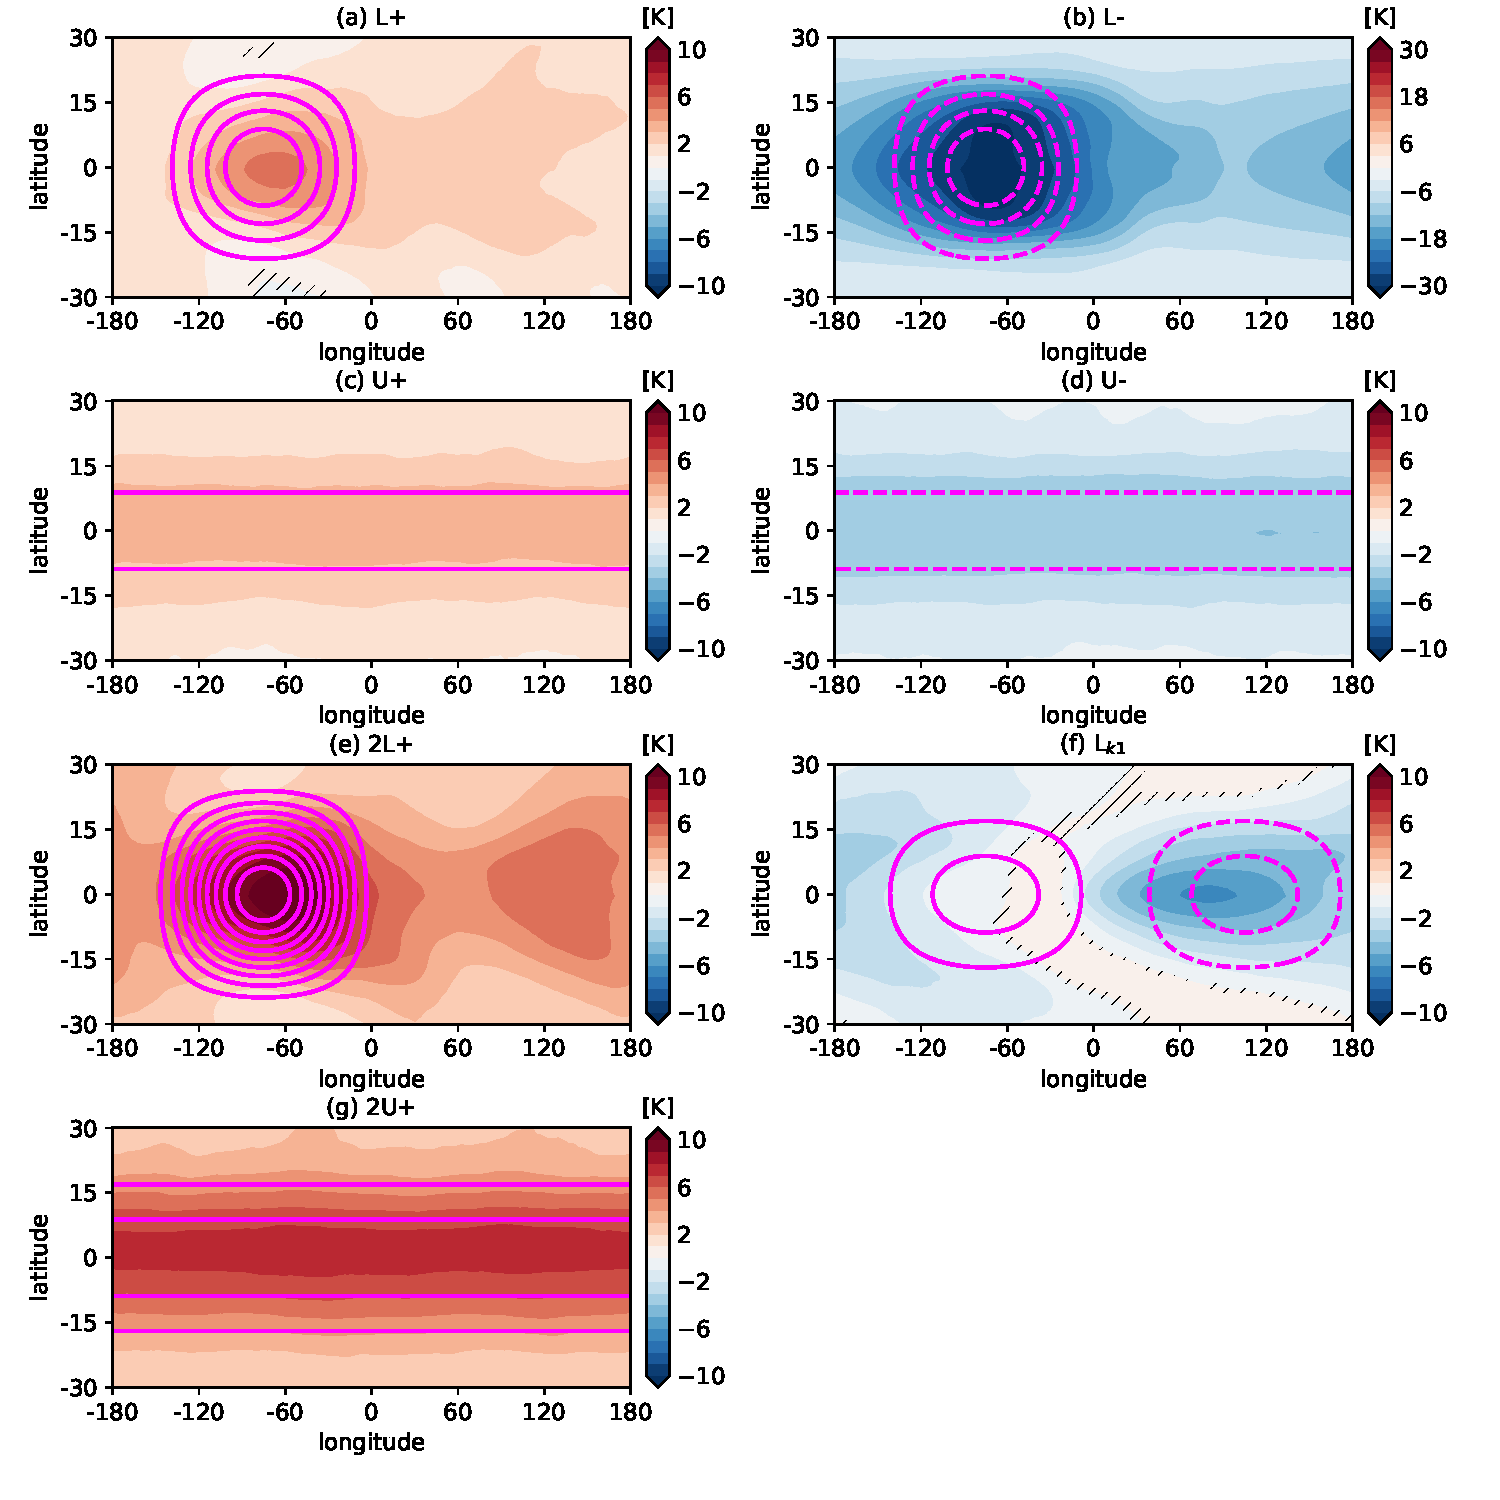
\includegraphics[trim=0cm 0cm 0cm 0cm, clip=true,scale=0.6]{./fig_01.pdf}\\
  \caption{Annual-mean tropical SST anomalies defined relative to the control simulation for experiments L+, L-, U+, U-, 2L+, L$_{k1}$ and 2U+ (see section 2 for description of the experiments). Purple contours denote Q-flux perturbations imposed in each experiment\cledit{,} with contour interval 30 Wm$^{-2}$ and solid lines denoting positive perturbations, and dashed lines denoting negative perturbations. Statistical significance is calculated at the 95 $\%$ level using a two-tailed student's $t$-test and hatching indicates anomalies that are not statistically significant. Note the different color bar range for experiment L- and that the fields in all experiments are phase shifted westwards by 75$^{\circ}$ for ease of viewing.}\label{f1}
\end{figure}

\newpage
\begin{figure}[ht]
  \noindent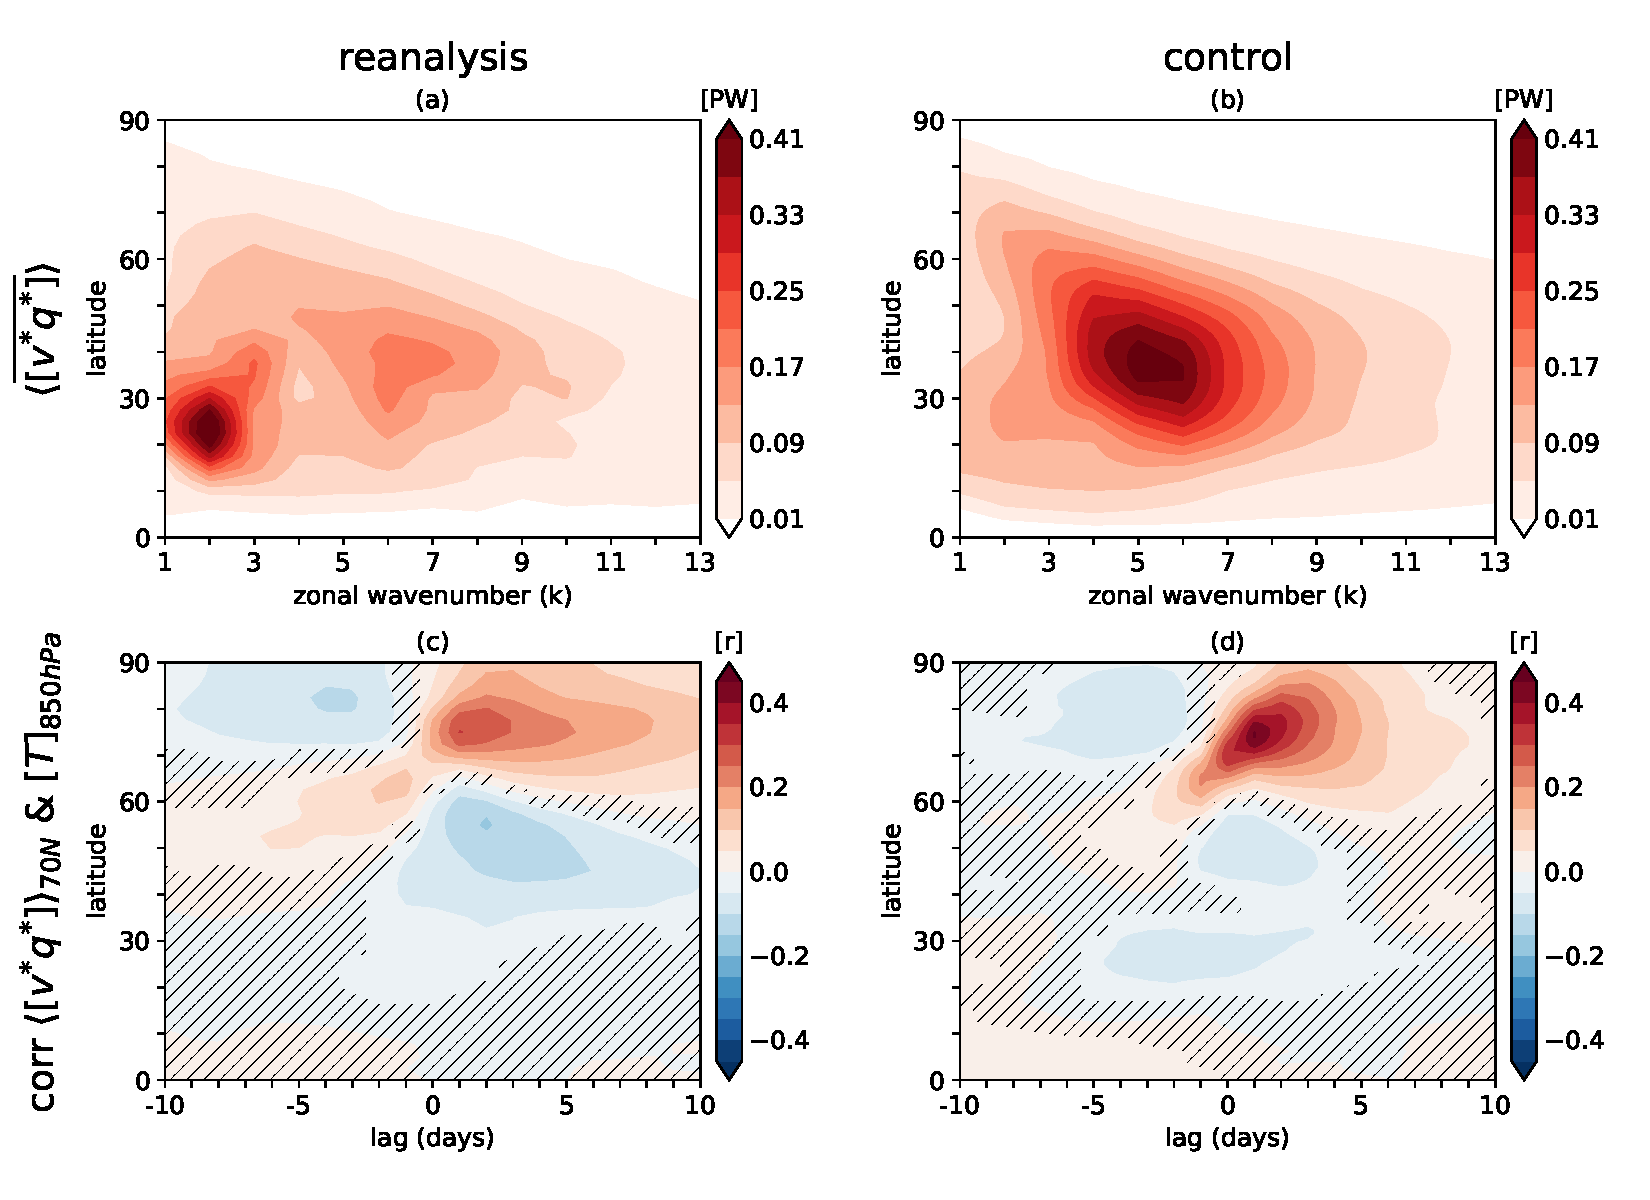
\includegraphics[trim=0cm 0cm 0cm 0cm, clip=true,scale=0.5]{./fig_02.pdf}\\
  \caption{(a,b) Annual-mean vertically and zonally integrated eddy moisture transport as a function of zonal wavenumber and latitude in (a) reanalysis and (b) the control simulation. The transport is multiplied by the latent heat of vaporization to give PW units. (c,d) Lag correlation between daily anomalies in zonal-mean temperature at 850 hPa and zonally and vertically integrated eddy moisture transport at 70$^{\circ}$N as a function of latitude. Anomalies are defined as deviations from the daily-mean seasonal cycle. Statistical significance is calculated at the 99$\%$ level with 5000 bootstrapped time series following the Monte-Carlo approach of \citeA{Ebisuzaki1997}. Hatching indicates correlations that are not statistically significant.}\label{f2}
\end{figure}


\newpage
\begin{figure}[ht]
  \noindent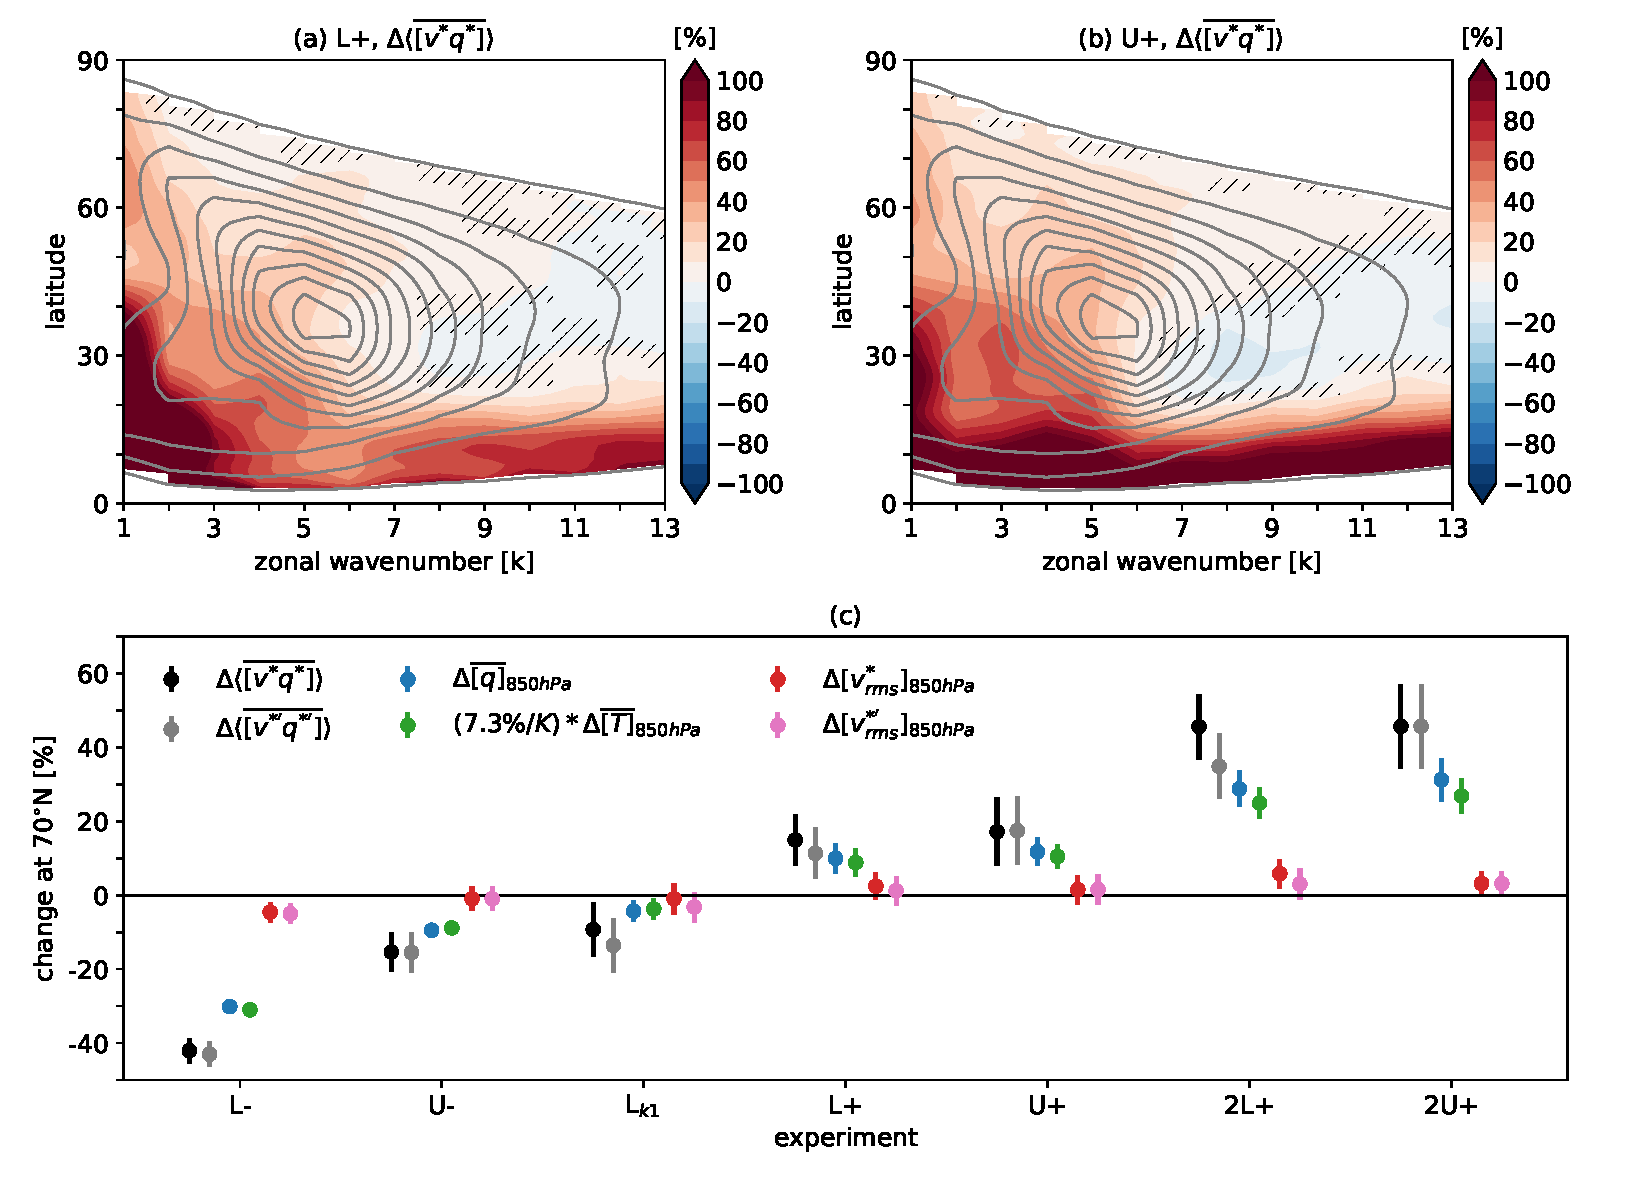
\includegraphics[trim=0cm 0cm 0cm 0cm, clip=true,scale=0.5]{./fig_03.pdf}\\
  \caption{(a,b) Annual-mean vertically and zonally integrated eddy moisture transport as a function of zonal wavenumber and latitude for the control simulation (contours) and percentage change from control for the L+ (local warming) and U+ (uniform warming) experiments (shading). Control contour interval is 0.04 PW starting at 0.01 PW and the percent change is shown where the climatology is greater than 0.01 PW. Statistical significance is calculated at the 95 $\%$ level using a two-tailed student's $t$-test and percent changes that are not statistically significant are hatched. (c)  Percentage change from control of the following annual-mean variables at 70$^{\circ}$N for all warming (+) and cooling (-) experiments: (black) vertically and zonally integrated eddy moisture transport, (gray) vertically and zonally integrated transient eddy moisture transport, (blue) zonal-mean specific humidity at 850 hPa, (red) zonal-mean root-mean-square eddy meridional wind at 850 hPa and (pink) zonal-mean root-mean square transient eddy meridional wind at 850 hPa. Green circles show the moisture transport change estimated from Clausius-Clapeyron scaling: zonal-mean temperature change in each experiment multiplied by 7.3 $\%/$K calculated from the control simulation \cite<equations 1 and 2 in>{HeldSoden2006}. Error bars denote the 95$\%$ inter-annual uncertainty range. The experiments are ordered by increasing temperature change at 70$^{\circ}$N from left to right.}\label{f3}
\end{figure}




%% ------------------------------------------------------------------------ %%
%% References and Citations

%%%%%%%%%%%%%%%%%%%%%%%%%%%%%%%%%%%%%%%%%%%%%%%
%
% \bibliography{<name of your .bib file>} don't specify the file extension
%
% don't specify bibliographystyle
%%%%%%%%%%%%%%%%%%%%%%%%%%%%%%%%%%%%%%%%%%%%%%%

\bibliography{references.bib}



%Reference citation instructions and examples:
%
% Please use ONLY \cite and \citeA for reference citations.
% \cite for parenthetical references
% ...as shown in recent studies (Simpson et al., 2019)
% \citeA for in-text citations
% ...Simpson et al. (2019) have shown...
%
%
%...as shown by \citeA{jskilby}.
%...as shown by \citeA{lewin76}, \citeA{carson86}, \citeA{bartoldy02}, and \citeA{rinaldi03}.
%...has been shown \cite{jskilbye}.
%...has been shown \cite{lewin76,carson86,bartoldy02,rinaldi03}.
%... \cite <i.e.>[]{lewin76,carson86,bartoldy02,rinaldi03}.
%...has been shown by \cite <e.g.,>[and others]{lewin76}.
%
% apacite uses < > for prenotes and [ ] for postnotes
% DO NOT use other cite commands (e.g., \citet, \citep, \citeyear, \nocite, \citealp, etc.).
%



\end{document}



More Information and Advice:

%% ------------------------------------------------------------------------ %%
%
%  SECTION HEADS
%
%% ------------------------------------------------------------------------ %%

% Capitalize the first letter of each word (except for
% prepositions, conjunctions, and articles that are
% three or fewer letters).

% AGU follows standard outline style; therefore, there cannot be a section 1 without
% a section 2, or a section 2.3.1 without a section 2.3.2.
% Please make sure your section numbers are balanced.
% ---------------
% Level 1 head
%
% Use the \section{} command to identify level 1 heads;
% type the appropriate head wording between the curly
% brackets, as shown below.
%
%An example:
%\section{Level 1 Head: Introduction}
%
% ---------------
% Level 2 head
%
% Use the \subsection{} command to identify level 2 heads.
%An example:
%\subsection{Level 2 Head}
%
% ---------------
% Level 3 head
%
% Use the \subsubsection{} command to identify level 3 heads
%An example:
%\subsubsection{Level 3 Head}
%
%---------------
% Level 4 head
%
% Use the \subsubsubsection{} command to identify level 3 heads
% An example:
%\subsubsubsection{Level 4 Head} An example.
%
%% ------------------------------------------------------------------------ %%
%
%  IN-TEXT LISTS
%
%% ------------------------------------------------------------------------ %%
%
% Do not use bulleted lists; enumerated lists are okay.
% \begin{enumerate}
% \item
% \item
% \item
% \end{enumerate}
%
%% ------------------------------------------------------------------------ %%
%
%  EQUATIONS
%
%% ------------------------------------------------------------------------ %%

% Single-line equations are centered.
% Equation arrays will appear left-aligned.

Math coded inside display math mode \[ ...\]
 will not be numbered, e.g.,:
 \[ x^2=y^2 + z^2\]

 Math coded inside \begin{equation} and \end{equation} will
 be automatically numbered, e.g.,:
 \begin{equation}
 x^2=y^2 + z^2
 \end{equation}


% To create multiline equations, use the
% \begin{eqnarray} and \end{eqnarray} environment
% as demonstrated below.
\begin{eqnarray}
  x_{1} & = & (x - x_{0}) \cos \Theta \nonumber \\
        && + (y - y_{0}) \sin \Theta  \nonumber \\
  y_{1} & = & -(x - x_{0}) \sin \Theta \nonumber \\
        && + (y - y_{0}) \cos \Theta.
\end{eqnarray}

%If you don't want an equation number, use the star form:
%\begin{eqnarray*}...\end{eqnarray*}

% Break each line at a sign of operation
% (+, -, etc.) if possible, with the sign of operation
% on the new line.

% Indent second and subsequent lines to align with
% the first character following the equal sign on the
% first line.

% Use an \hspace{} command to insert horizontal space
% into your equation if necessary. Place an appropriate
% unit of measure between the curly braces, e.g.
% \hspace{1in}; you may have to experiment to achieve
% the correct amount of space.


%% ------------------------------------------------------------------------ %%
%
%  EQUATION NUMBERING: COUNTER
%
%% ------------------------------------------------------------------------ %%

% You may change equation numbering by resetting
% the equation counter or by explicitly numbering
% an equation.

% To explicitly number an equation, type \eqnum{}
% (with the desired number between the brackets)
% after the \begin{equation} or \begin{eqnarray}
% command.  The \eqnum{} command will affect only
% the equation it appears with; LaTeX will number
% any equations appearing later in the manuscript
% according to the equation counter.
%

% If you have a multiline equation that needs only
% one equation number, use a \nonumber command in
% front of the double backslashes (\\) as shown in
% the multiline equation above.

% If you are using line numbers, remember to surround
% equations with \begin{linenomath*}...\end{linenomath*}

%  To add line numbers to lines in equations:
%  \begin{linenomath*}
%  \begin{equation}
%  \end{equation}
%  \end{linenomath*}



